\chapter{Experimentación}
\hrule \bigskip \vspace*{1cm}
%------------------------------------------------------------------------

En este capítulo describiremos la aplicación de una de las técnicas de clasificación como parte del aprendizaje supervisado basado en corpus. Para ello se han tomado dos fuentes de entrenamiento, una de elaboración propia (en español) y otra fuente disponible en el sitio \emph{Web} kaggle.com (en inglés).

La fuente de elaboración propia contiene porciones extraídas del resumen de usuarios que exponen su perfil profesional en un sitio especializado como LinkedIn. Para la fase de entrenamiento se espera clasificar perfiles que coinciden con el perfil de "Analista Programador" y diferenciarlos de otros como por ejemplo "Analista Funcional" o "Analista de Planeamiento", entre otros.

Con respecto a la fuente descargada en inglés, ésta contiene tweets con mensajes ofensivos y no ofensivos. Al estar en un sitio público, ésta contiene mayor cantidad de datos de entrenamiento, lo cual permite lograr un mejor entrenamiento durante la fase de aprendizaje.

\section{Procedimiento}

Como algoritmo de clasificación se utilizó kNN (k-Nearest Neighbors). El procedimiento aplicado para la clasificación y pronóstico de textos mostrado en la figura \ref{fig:experimentacion} inicia con el entrenamiento del modelo, para ello se requiere de una fuente de datos previamente etiquetada. En la fase de predicción, se prueba el modelo con un conjunto de textos distinto al inicial (conjunto de prueba), el cual también está etiquetado para su verificación posterior.

Finalmente el resultado (conjunto de predicciones) se compara con el valor esperado del conjunto de prueba para el análisis respectivo.


\begin{figure}[h!]
	\begin{center}
	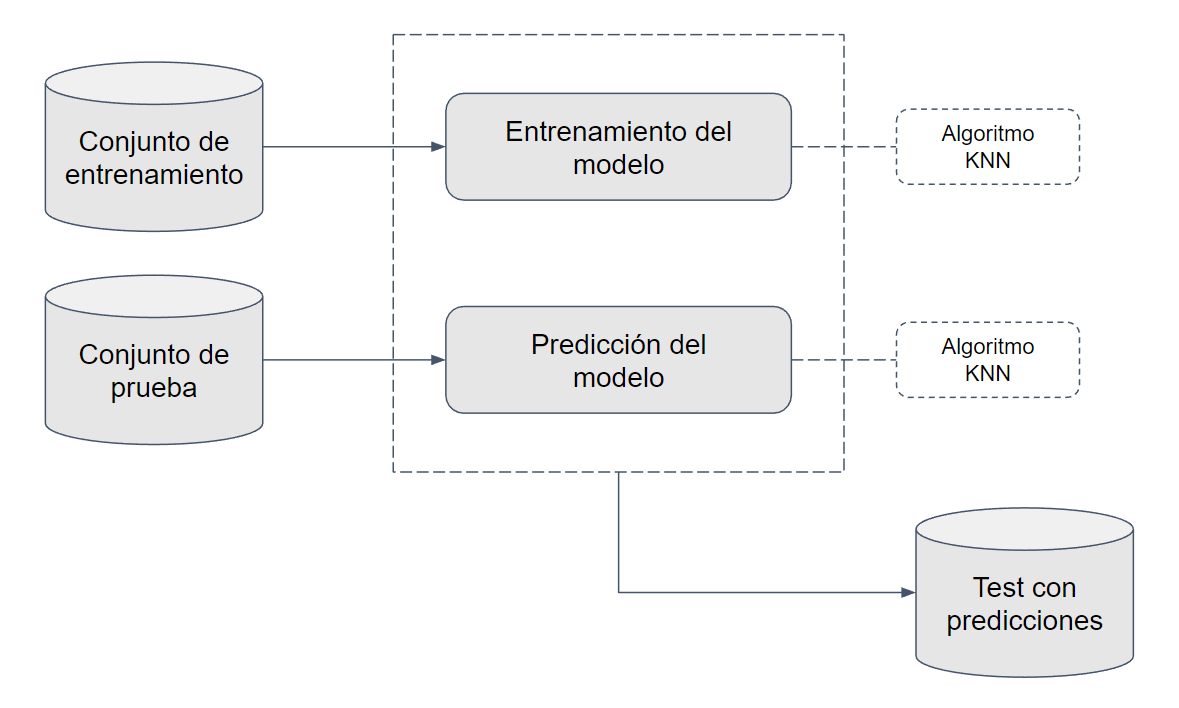
\includegraphics[angle=0,width=9.5cm]{Graficos/experimentacion1}
	\caption{Procedimiento aplicado para del método de clasificación.}
	\label{fig:experimentacion}
  \end{center}
\end{figure}

\section{Tratamiento del texto}

\subsection{Bolsa de palabras}

En esta primera fase, el texto de entrada pasa por un proceso inicial de preparación (tokenización), luego se procede a extraer características del texto (diccionario) y la frecuencia de cada una. Finalmente el diccionario de palabras se transforma en un vector de características para cada entrada (frase o tweet). La figura \ref{fig:bolsa} muestra este proceso con los resultados de forma visual.

Durante la tokenización, se extraen símbolos y carácteres no reconocibles. En el caso de los tweets, hay mayor cantidad de textos no reconocibles al provenir de una fuente de mensajería informal (se utilizan abreviaciones, emojis, o repeticiones de algunas letras, por ejemplo: 'awwwwww', 'noooo', 'lol', 'xD').

Teniendo el texto libre de símbolos extraños, se procede a extraer un diccionario de palabras con su respectiva frecuencia, tal como se muestra en la segunda parte de la figura \ref{fig:bolsa}. Este diccionario sirve para convertir cada texto de entrada en un vector de características, donde cada elemento del mismo representa la cantidad de veces que aparece una palabra determinada en el texto. Este vector es de N dimensiones, contiene muchos ceros (palabras que no aparecen en el texto), por lo cual es conveniente aplicar algún método de reducción de dimensionalidad.

\begin{figure}[h!]
	\begin{center}
	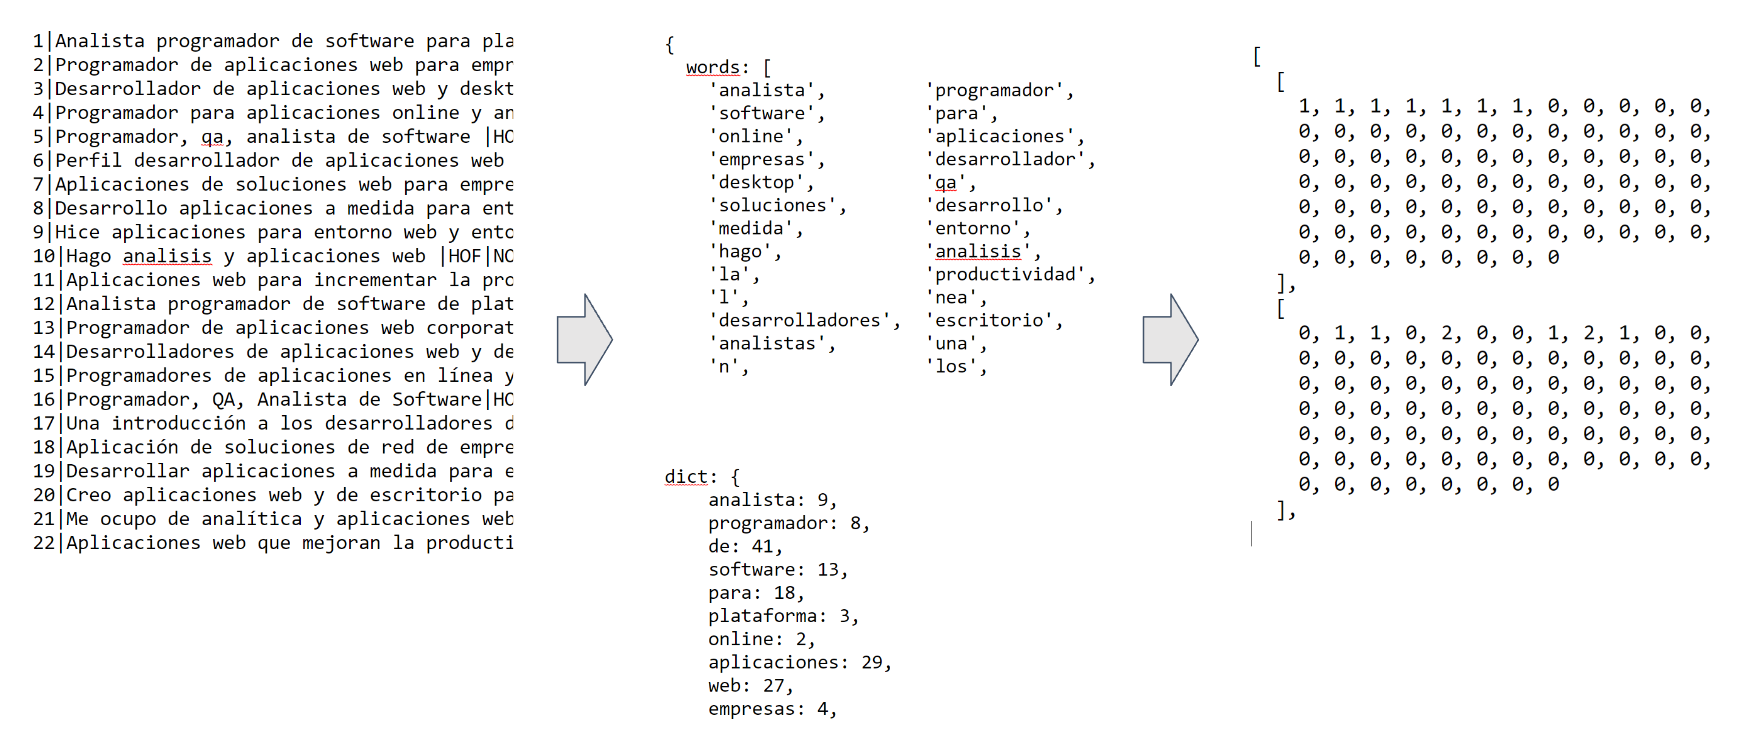
\includegraphics[angle=0,width=9.5cm]{Graficos/bolsa_palabras}
	\caption{Tratamiento del texto al aplicar la bolsa de palabras.}
	\label{fig:bolsa}
  \end{center}
\end{figure}

\subsection{Reducción de dimensiones}

El vector de características que se obtiene luego de aplicar la Bolsa de Palabras, es de N dimensiones, dependiendo de qué tan grande es el diccionario generado. Cuanto más grande sea la variedad de palabras mayor será el tamaño del diccionario y en consecuencia el tamaño del vector generado.

Aplicar un algoritmo de clasificación sobre este vector de N dimensiones no es aconsejable, por el procesamiento alto que conlleva trabajar de N dimensiones; en ese sentido, es necesario reducir la dimensionalidad de dicho vector.

Para este experimento, se aplica el algoritmo MDS (\emph{Multidimensional Scaling}) cuyo detalle se explicó en la sección \ref{mds}. Para efectos prácticos, se aplicó una reducción a 2 dimensiones. La figura \ref{fig:mds} muestra el resultado luego de aplicar el algoritmo al vector N-dimensional resultado de la bolsa de palabras.

\begin{figure}[h!]
	\begin{center}
	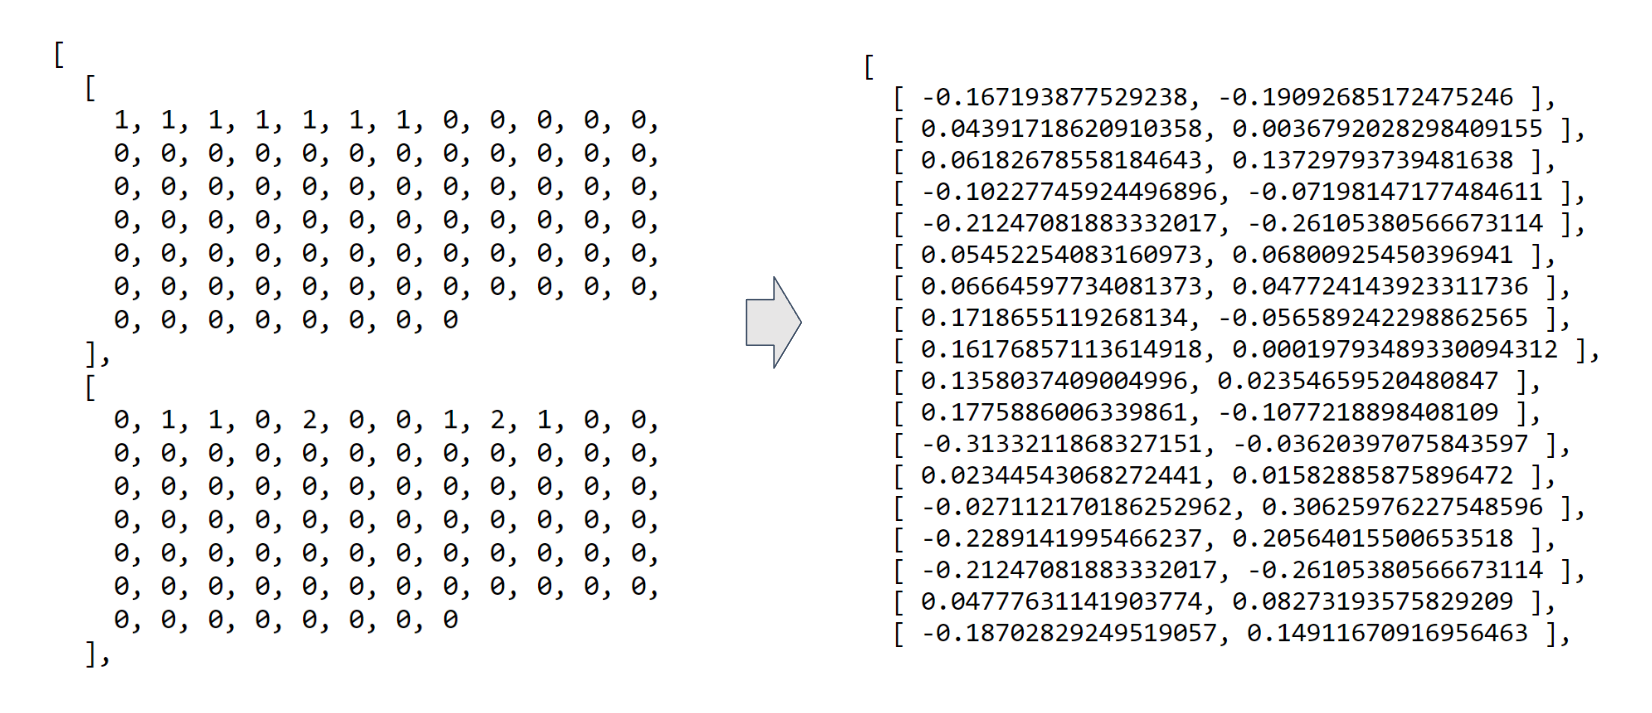
\includegraphics[angle=0,width=9.5cm]{Graficos/mds}
	\caption{Reducción de dimensiones aplicando el algoritmo MDS.}
	\label{fig:mds}
  \end{center}
\end{figure}

\subsection{Reducción de dimensiones}

El vector de características que se obtiene luego de aplicar la Bolsa de Palabras, es de N dimensiones, dependiendo de qué tan grande es el diccionario generado. Cuanto más grande sea la variedad de palabras mayor será el tamaño del diccionario y en consecuencia el tamaño del vector generado.

Aplicar un algoritmo de clasificación sobre este vector de N dimensiones no es aconsejable, por el procesamiento alto que conlleva trabajar de N dimensiones; en ese sentido, es necesario reducir la dimensionalidad de dicho vector.

Para este experimento, se aplica el algoritmo MDS (\emph{Multidimensional Scaling}) cuyo detalle se explicó en la sección \ref{mds}. Para efectos prácticos, se aplicó una reducción a 2 dimensiones. La figura \ref{fig:mds} muestra el resultado luego de aplicar el algoritmo al vector N-dimensional resultado de la bolsa de palabras.

\begin{figure}[h!]
	\begin{center}
	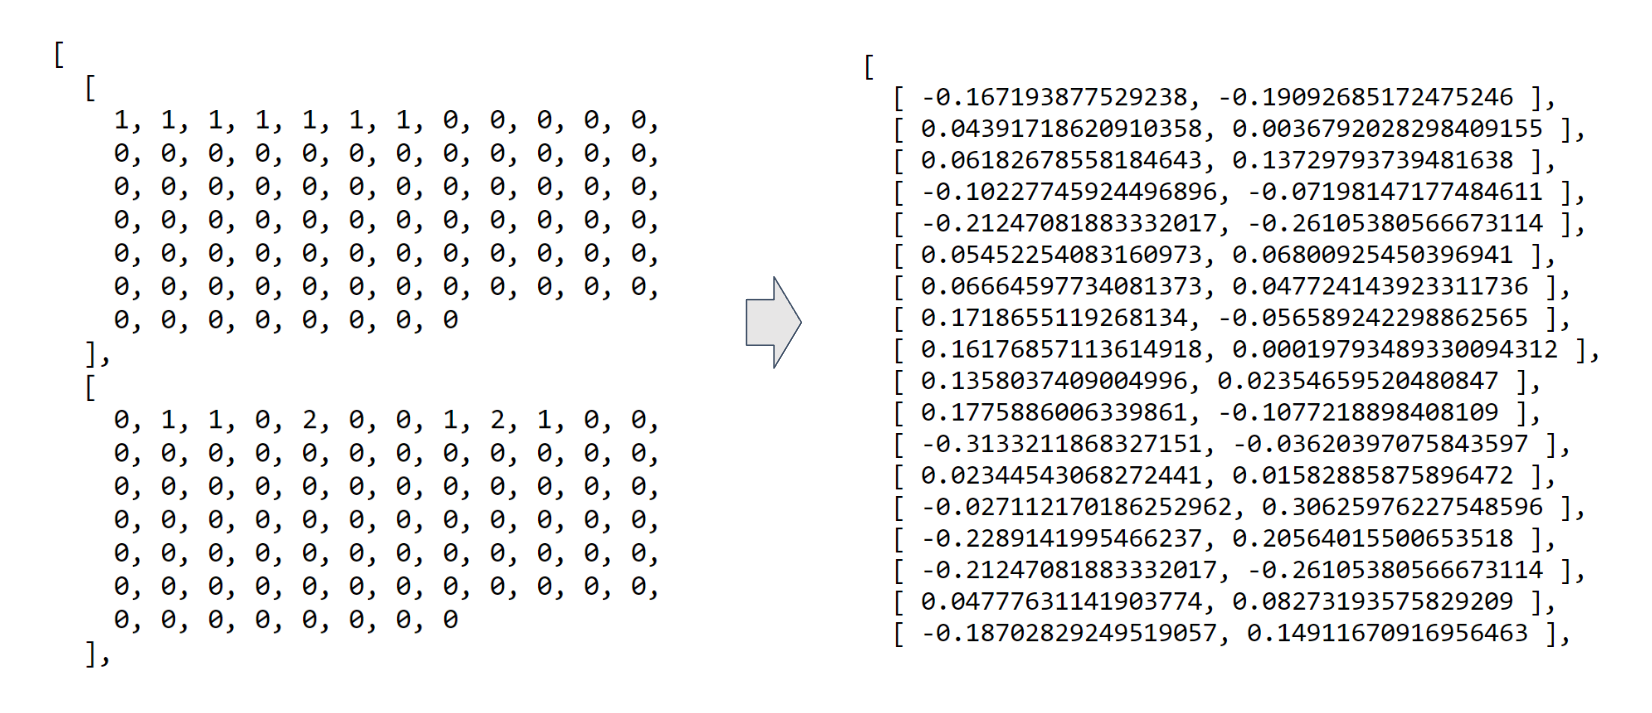
\includegraphics[angle=0,width=9.5cm]{Graficos/mds}
	\caption{Reducción de dimensiones aplicando el algoritmo MDS.}
	\label{fig:mds}
  \end{center}
\end{figure}

\subsection{Clasificación y entrenamiento}

Como se mencionó anteriormente, el algoritmo de clasificación utilizado es el \emph{kNN}. Su implementación está basada en una estructura \emph{KD Tree} y se escogió un valor de $k = 7$ para el experimento. De esta forma se seleccionarán los 7 vecinos más cercanos para clasificar los nuevos mensajes.

La figura \ref{fig:knn_train} la distribución de puntos en 2D, diferenciando las clases en color rojo y verde. Para el conjuntos de entrenamiento relacionados a tweets, en inglés, se muestran en color verde los tweets clasificados como no ofensivos y en rojo los ofensivos. Para el conjunto de entrenamiento relacionados a resúmenes de perfil profesional, en verde los textos relacionados a un perfil de Analista Programador o Desarrolladores, y en rojo los que están relacionados a otro perfil.

Los resultados se muestran en la figura \ref{fig:knn_train_results}. La aplicación del algoritmo sobre el conjunto de prueba es un conjunto de vectores con la posición final de cada punto y la clasificación respectiva, hecha en base a los k vecinos más cercanos ($k = 7$);

Finalmente, cuando se pretende evaluar un mensaje nuevo, se muestra un punto de color negro y el resultado de la clasificación.

\begin{figure}[h!]
	\begin{center}
	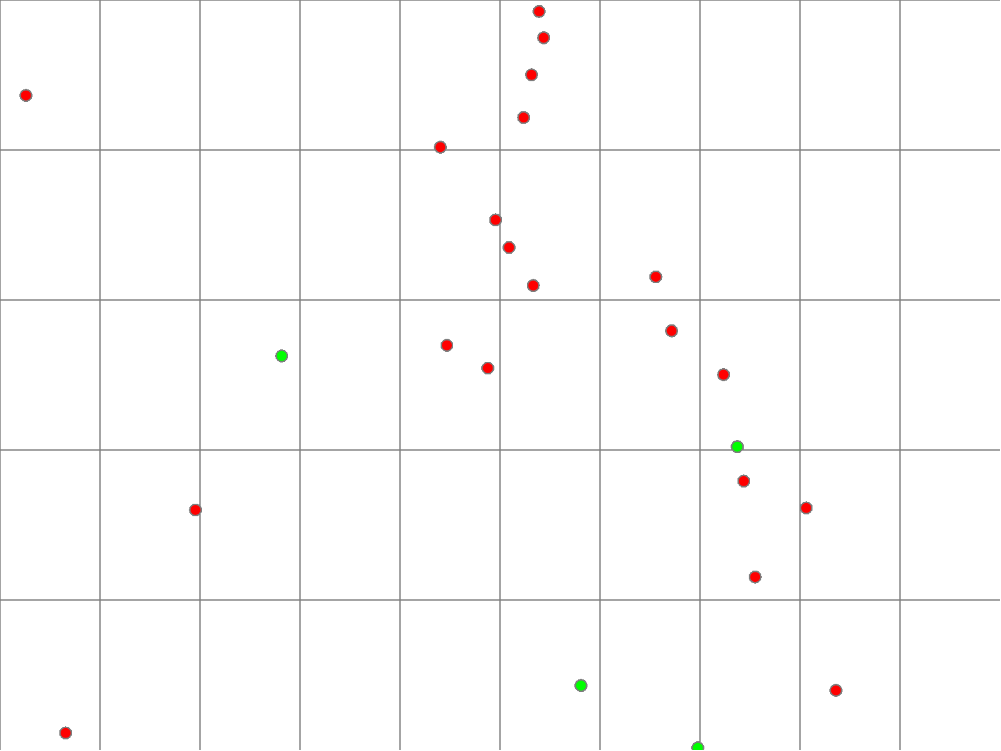
\includegraphics[angle=0,width=9.5cm]{Graficos/knn_train}
	\caption{Clasificación de mensajes de entrenamiento.}
	\label{fig:knn_train}
  \end{center}
\end{figure}


\begin{figure}[h!]
	\begin{center}
	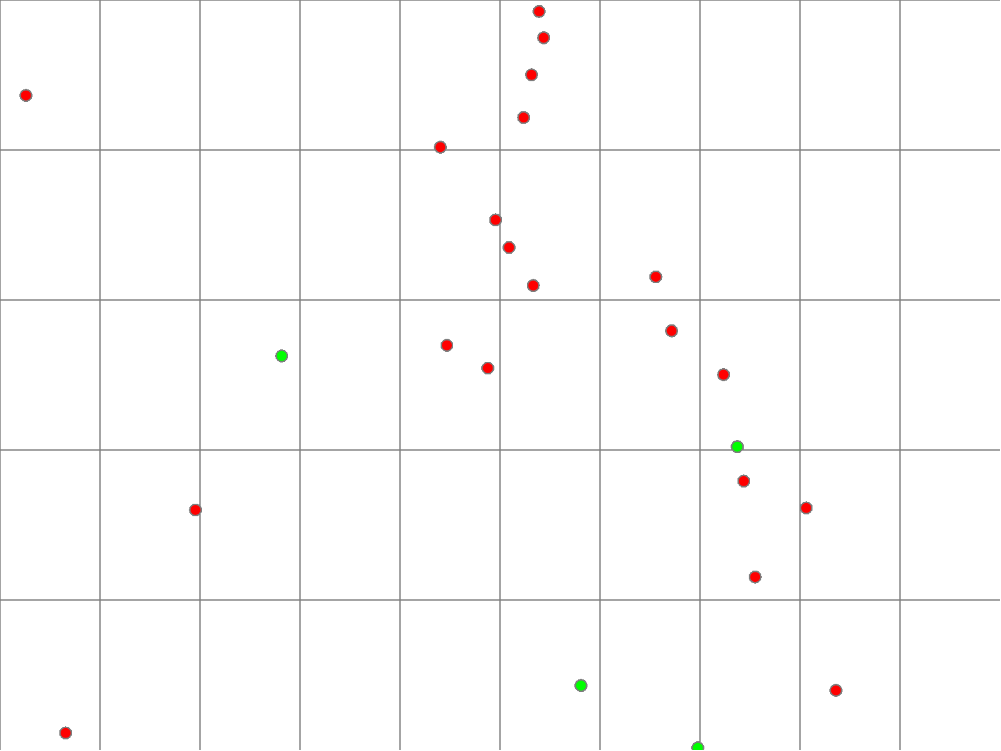
\includegraphics[angle=0,width=9.5cm]{Graficos/knn_train_results}
	\caption{Clasificación de mensajes de entrenamiento.}
	\label{fig:knn_train_results}
  \end{center}
\end{figure}


\section{Resultados}

En la figura  \ref{fig:knn_experimento}  \label[ss]{} en la parte (A) mostramos los puntos en negro a ser clasificados por nuestro algoritmo, en la parte (B) mostramos el resultado luego de la clasificación.


\begin{figure}[h!]
	\begin{center}
	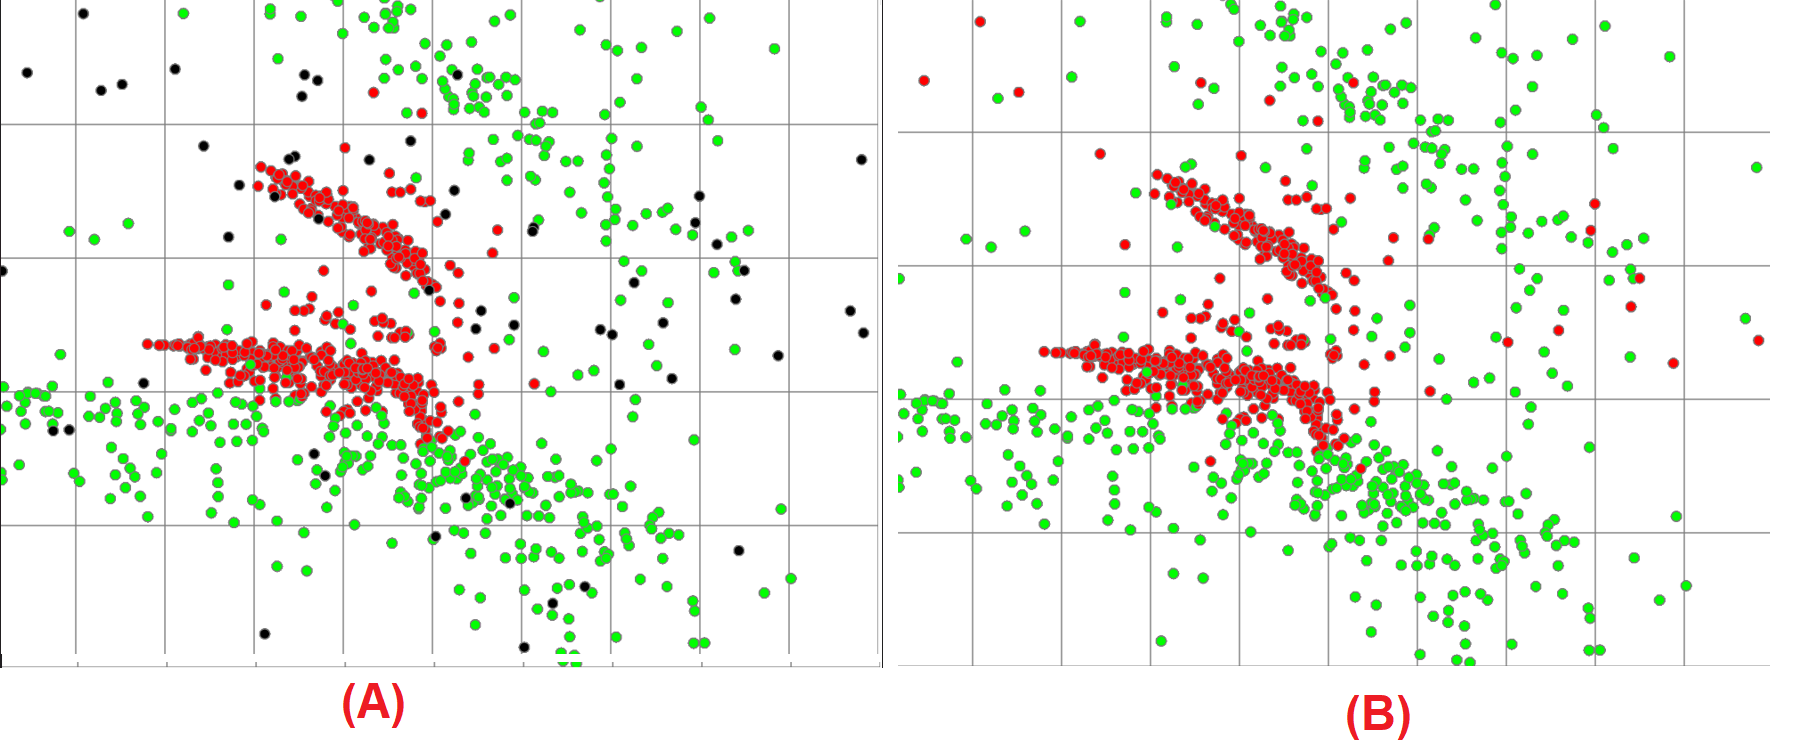
\includegraphics[ width=15cm]{Graficos/Comparacion1}
	\caption{Resultado después de la prueba  }
	\label{fig:knn_experimento}
  \end{center}
\end{figure}
